\subsubsection{biguint-sub}
\label{biguint-sub}

\begin{enumerate}
    \item target
        implenmet the substraction of two biguints.
    \item constraints-logic
        \begin{itemize}
            \item equation for gate
            \item sumcheck for ouptput 
            \item rangecheck for limbs
        \end{itemize}
    \item circuit layout
        \begin{figure}[!ht]
            \centering
            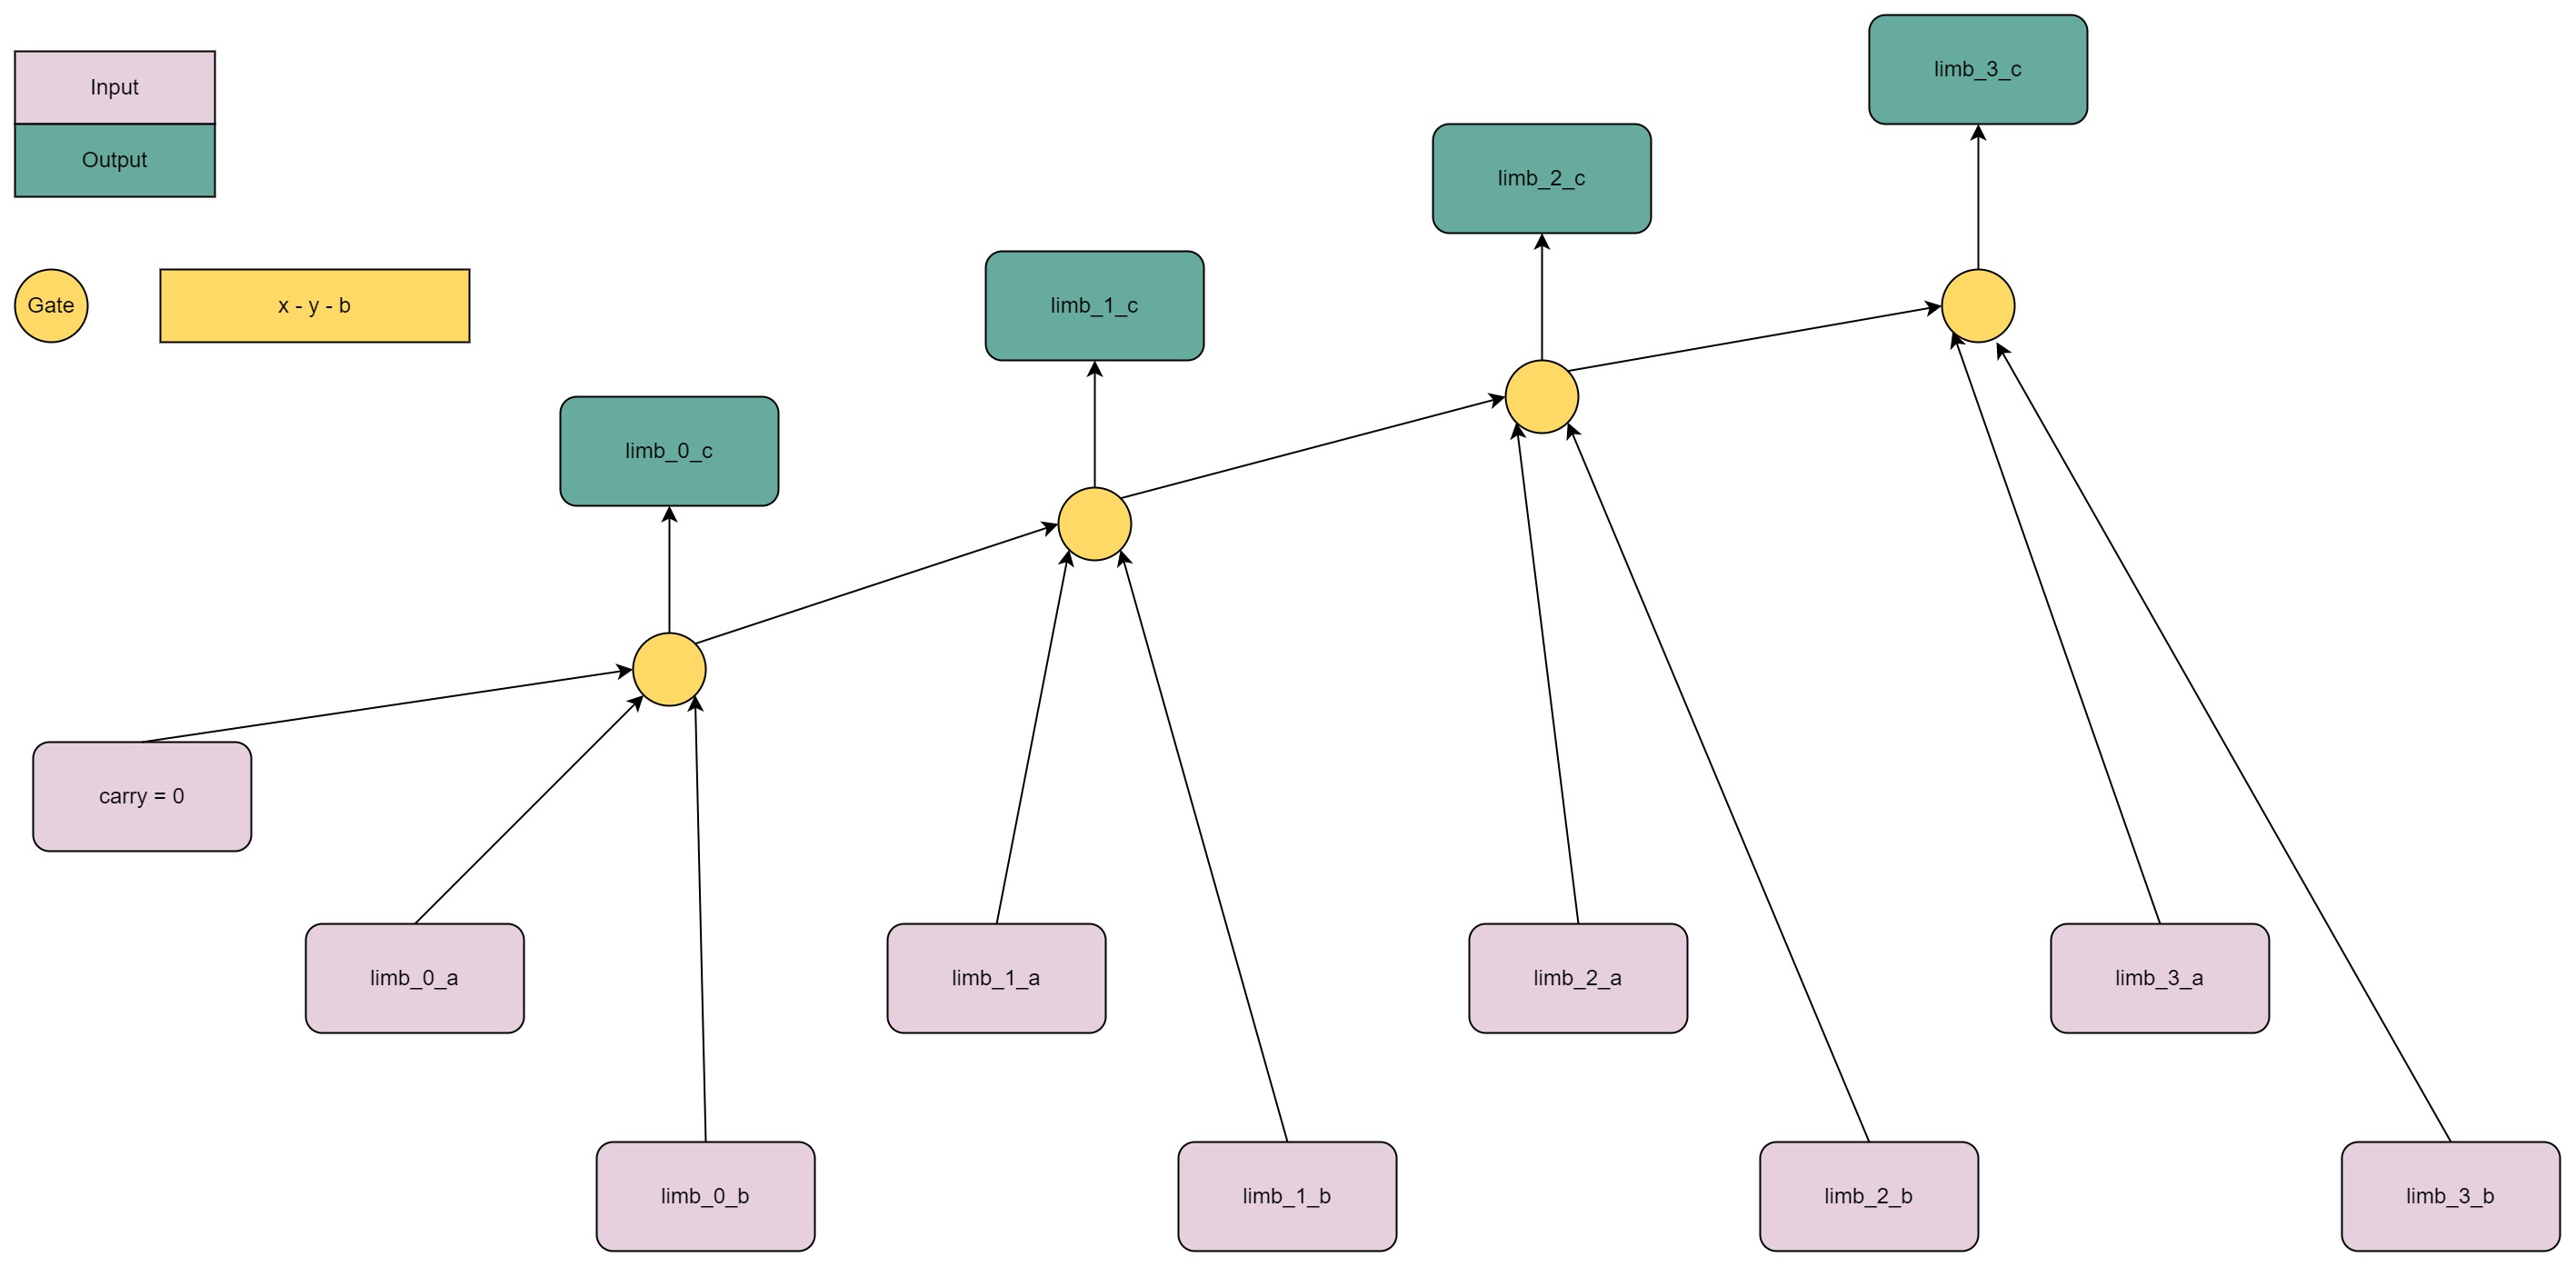
\includegraphics[width=0.8\textwidth]{biguint-sub-circuit-layout.jpg}
            \caption{biguint-sub circuit layout}
            \label{fig:biguint-sub-circuit-layout}
        \end{figure}

    \item trace layout
        \begin{figure}[!ht]
            \centering
            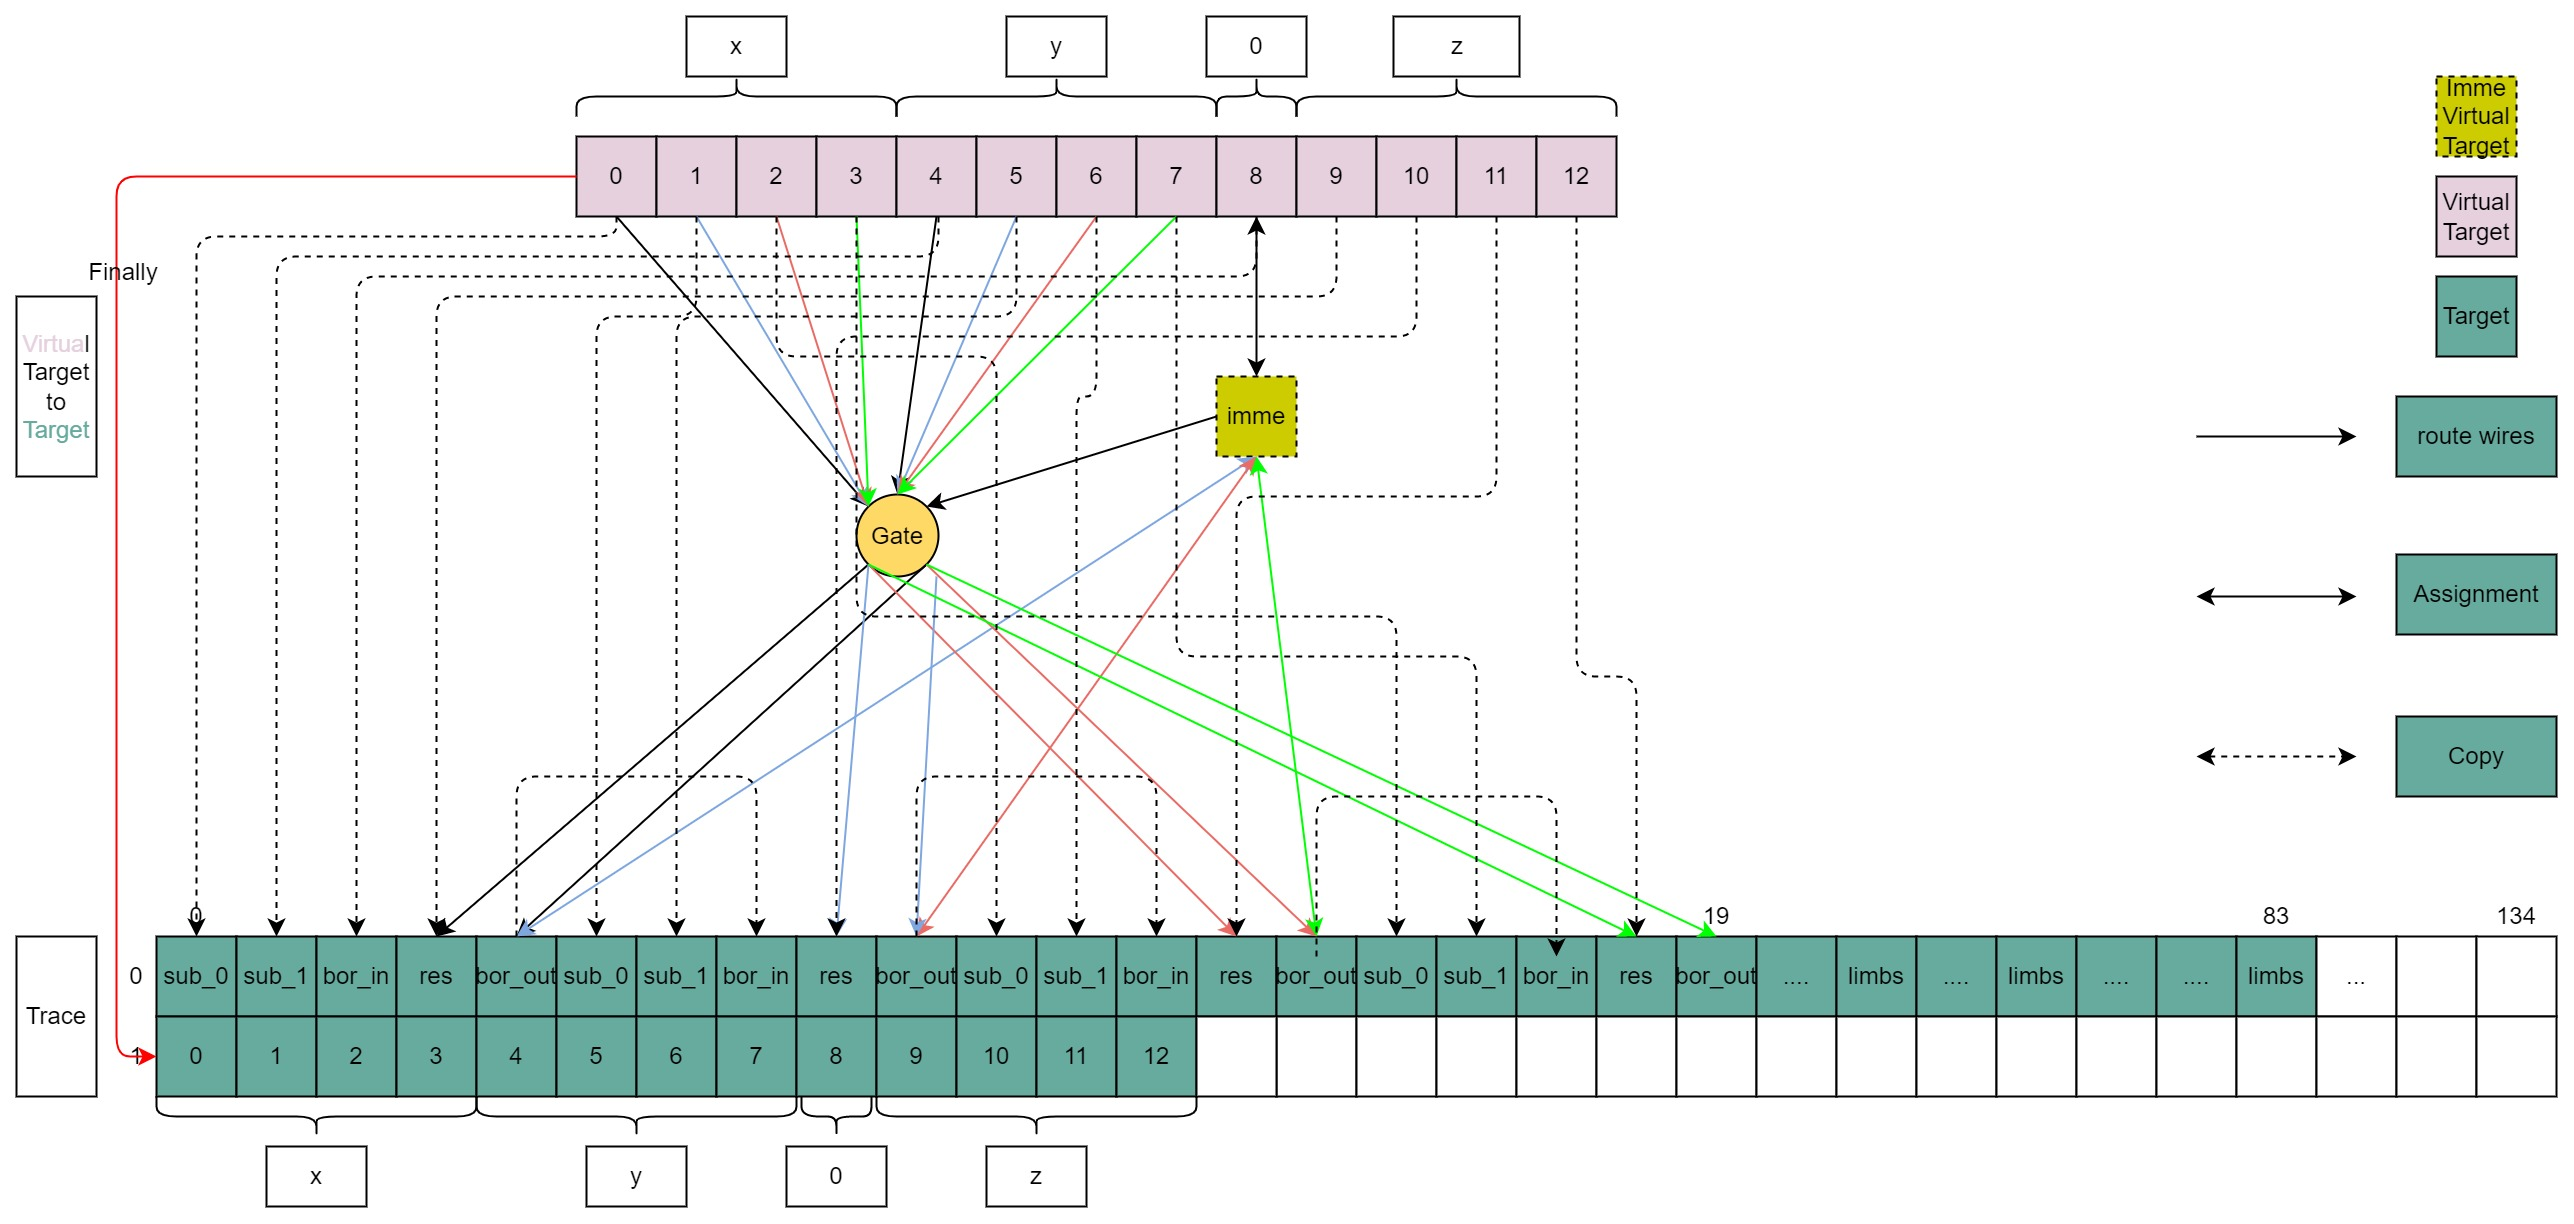
\includegraphics[width=0.8\textwidth]{biguint-sub-trace-layout.jpg}
            \caption{biguint-sub trace layout}
            \label{fig:biguint-sub-trace-layout}
        \end{figure}
    
    \item constraints-info and costs
        \begin{itemize}
            \item constraints-num: 6 * (3 + 32 / 2) = 114
            \item copy-constraints: 16
            \item max-degree: 4
            \item wires-num: 6 * (5 + 16) = 126
        \end{itemize}

    \item questions
        \begin{itemize}
            \item why not make rangecheck constraint for inputs?
            \item Could try to use the same constraint with add-gate.
        \end{itemize}

\end{enumerate}